\documentclass[10pt, oneside]{article}
\usepackage[a4paper, total={5.5in, 9in}]{geometry}
\usepackage[ngerman]{babel}

\usepackage{blindtext}
\usepackage{titlesec}
\usepackage{amsmath}
\usepackage[hidelinks]{hyperref}
\usepackage{parskip}
\usepackage{graphicx}
\usepackage{longtable}
\usepackage[shortlabels]{enumitem}
\usepackage{multirow}
\usepackage{nccmath}
\usepackage{rotating}
\usepackage{makecell}
\usepackage{multicol}
\usepackage{capt-of}
\usepackage{csquotes}
\usepackage{amsfonts}
\usepackage{caption}

\captionsetup[table]{position=bottom}

\titleformat{\section}
    {\normalfont\Large\bfseries}{}{0pt}{}

\let\oldsection\section
\renewcommand{\section}{
  \renewcommand{\theequation}{\thesection.\arabic{equation}}
  \oldsection}
\let\oldsubsection\subsection
\renewcommand{\subsection}{
  \renewcommand{\theequation}{\thesubsection.\arabic{equation}}
  \oldsubsection}

\makeatletter
\renewcommand{\maketitle}{
    \bgroup
    \centering
    \par\LARGE\@title  \\[20pt]
    \par\large\@author \\[10pt]
    \par\large\@date
    \par
    \egroup
}
\makeatother


\title{Mathematische Grundlagen\\[10pt]\Large{WiSe 2024/25}}
\author{Volodymyr But\\[10pt]Hochschule Trier}
\date{}

% - - - - - - - - - - - - - - - - - - - - - - - - - - - - - - - - - - - - - - %

\begin{document}
\sloppy

\maketitle
\vspace{25px}

\section{Aufgabe 1}

Stellen Sie sich vor, Sie sind Teil eines Forschungsteams, das eine Studie
"uber das Essverhalten in Großst"adten durchf"uhrt. Ihre Untersuchungseinheiten
sind Einwohner einer Großstadt. F"ur jede Untersuchungseinheit werden folgende
Merkmale erfasst.

\begin{enumerate}[-]
    \item Alter (in Jahren)
    \item Berufsgruppe (z.B Lehrer, Ingenieur, Student, usw.)
    \item Monatliches Einkommen (in Euro)
    \item Durchschnittliche Ausgaben f"ur Lebensmittel pro Woche (in Euro)
    \item Bevorzugte Art von Restaurant
    \item H"aufigkeit des Restaurantbesuchs pro Monat
    \item Bewertung der eigenen Kochf"ahigkeiten (auf eine Skala von 1 bis 5,
        wobei 1 sehr schlecht und 5 ausgezeichnet bedeutet)
\end{enumerate}

Klassifizieren Sie jedes dieser Merkmale als quantitativ oder qualitativ.
Unterteilen Sie weiter die qualitativen Merkmale in nominale und ordinale
Merkmale.

\bgroup
\def\arraystretch{1.5}
\begin{table}[h]
    \centering
    \begin{tabular}{p{0.33\linewidth}|p{0.33\linewidth}|p{0.33\linewidth}}
        \hfil\multirow{2}{*}{\centering quantitativ} & \multicolumn{2}{c}{qualitativ} \\
        \cline{2-3}
        & \hfil nominale & \hfil ordinale \\ \hline
        Alter & Berufsgruppe & Bevorzugte Art von Restaurant \\ \cline{1-1} \cline{3-3}
        Monatliches Einkommen & & Bewertung der Kochf"ahigkeiten \\ \cline{1-1}
        Durchschnittliche Ausgaben pro Woche & & \\ \cline{1-1}
        H"aufigkeit des Restaurantbesuchs pro Monat & &
    \end{tabular}
\end{table}
\egroup

\section{Aufgabe 4}
\setcounter{section}{4}

\begin{enumerate}[(a)]
    \item \begin{enumerate}[i)]
            \item Finden Sie ein \textbf{Gegenbeispiel}, das zeigt, dass
                folgende Aussage allgemein \textbf{nicht} gilt: Seien
                $M,M_1,M_2$ nicht-leere Mengen, sodass $M_1 \subset M$,
                $M_2 \subset M$, $M_1 \cap M_2 = \emptyset$. Dann gilt auch
                $M_1 \cup M_2 = M$

                Es seien $M := \{ 1, 2, 3, 4, 5, 6, 7, 8, 9 \}$, $M_1 := \{1,
                2, 3, 4\}$, $M_2 := \{6, 7, 8, 9\}$. Dann gilt:
                $$M_1 \subset M, \quad M_2 \subset M, \quad M_1 \cap M_2 = \emptyset$$
                Dann gilt $M_1 \cup M_2 \neq M$, weil
                $$M_1 \cup M_2 = \{ 1, 2, 3, 4, 6, 7, 8, 9 \} \neq \{1, 2, 3, 4, \textbf{5}, 6, 7, 8, 9\} = M $$
                Die Aussage aus der Aufgabenstellung ist somit falsch.

            \item Geben Sie au{\ss}erdem ein Beispiel an, f"ur das die Aussage gilt.

                Es seien $M := \{ 1, 2, 3, 4, 5, 6, 7, 8, 9 \}$, $M_1 := \{1,
                2, 3, 4\}$, $M_2 := \{\textbf{5}, 6, 7, 8, 9\}$. Dann gilt:
                $$M_1 \subset M, \quad M_2 \subset M, \quad M_1 \cap M_2 = \emptyset$$
                wie auch
                $$M_1 \cup M_2 = \{1, 2, 3, 4, \textbf{5}, 6, 7, 8, 9\} = M$$

            \item Verbinden Sie $M, M_1, M_2$ mithilfe der
                Komplement-Mengeoperation zu einer Formel, die f"ur den Fall
                aus ii) gilt.

                Anhand des Beispiels aus ii) lässt sich feststellen, dass wenn
                $M,M_1,M_2$ nicht-leere Mengen sind, sodass $$M_1 \subset M,
                \quad M_2 \subset M, \quad M_1 \cap M_2 = \emptyset$$ gilt die
                Aussage $M_1 \cup M_2 = M$ nur wenn $$M_1^{c(M)} = M_2
                \quad\text{oder}\quad M_2^{c(M)} = M_1$$
        \end{enumerate}
    \item \begin{enumerate}[i)]
            \item  Schreiben Sie die folgende Menge in der beschreibenden Mengenschreibweise:
                Die Menge aller geordneter zwei-Tupel, wobei die erste
                Komponente eine ganze Zahl und die zweite Komponente eine n
                nat"urliche Zahl ungleich 0 ist und die beiden Zahlen sind
                teilerfremd.

                $$M = \{ (x_1, x_2) \in \mathbb{Z} \times \mathbb{N} : \text{ggT}(x_1, x_2) = 1\ \text{und}\ x_2 \neq 0 \}$$

            \item Welche allgemein bekannte Zahlen-Menge haben Sie gerade beschrieben?

                Die Menge aller vereinfachten Brüche
        \end{enumerate}
\end{enumerate}


\section{Aufgabe 6}
\setcounter{section}{6}

\begin{enumerate}[(a)]
    \item Skizzieren Sie die Menge $[-1, 3] \times \{-2,2,3\}$.

        \begin{align*}
            M = [-1, 3] \times \{-2,2,3\} &= \{-1, 0, 1, 2, 3\} \times \{-2, 2, 3\} = \\
                                          &=
                    \begin{aligned}[t]
                        \{&(-1, -2), (-1, 2), (-1, 3), (0, -2), (0, 2),\\
                          &(0, 3), (1, -2), (1, 2), (1, 3), (2, -2), (2, 2),\\
                          &(2, 3), (3, -2), (3, 2), (3, 3)\}
                    \end{aligned}
        \end{align*}

        \begin{figure}[h]
            \centering
            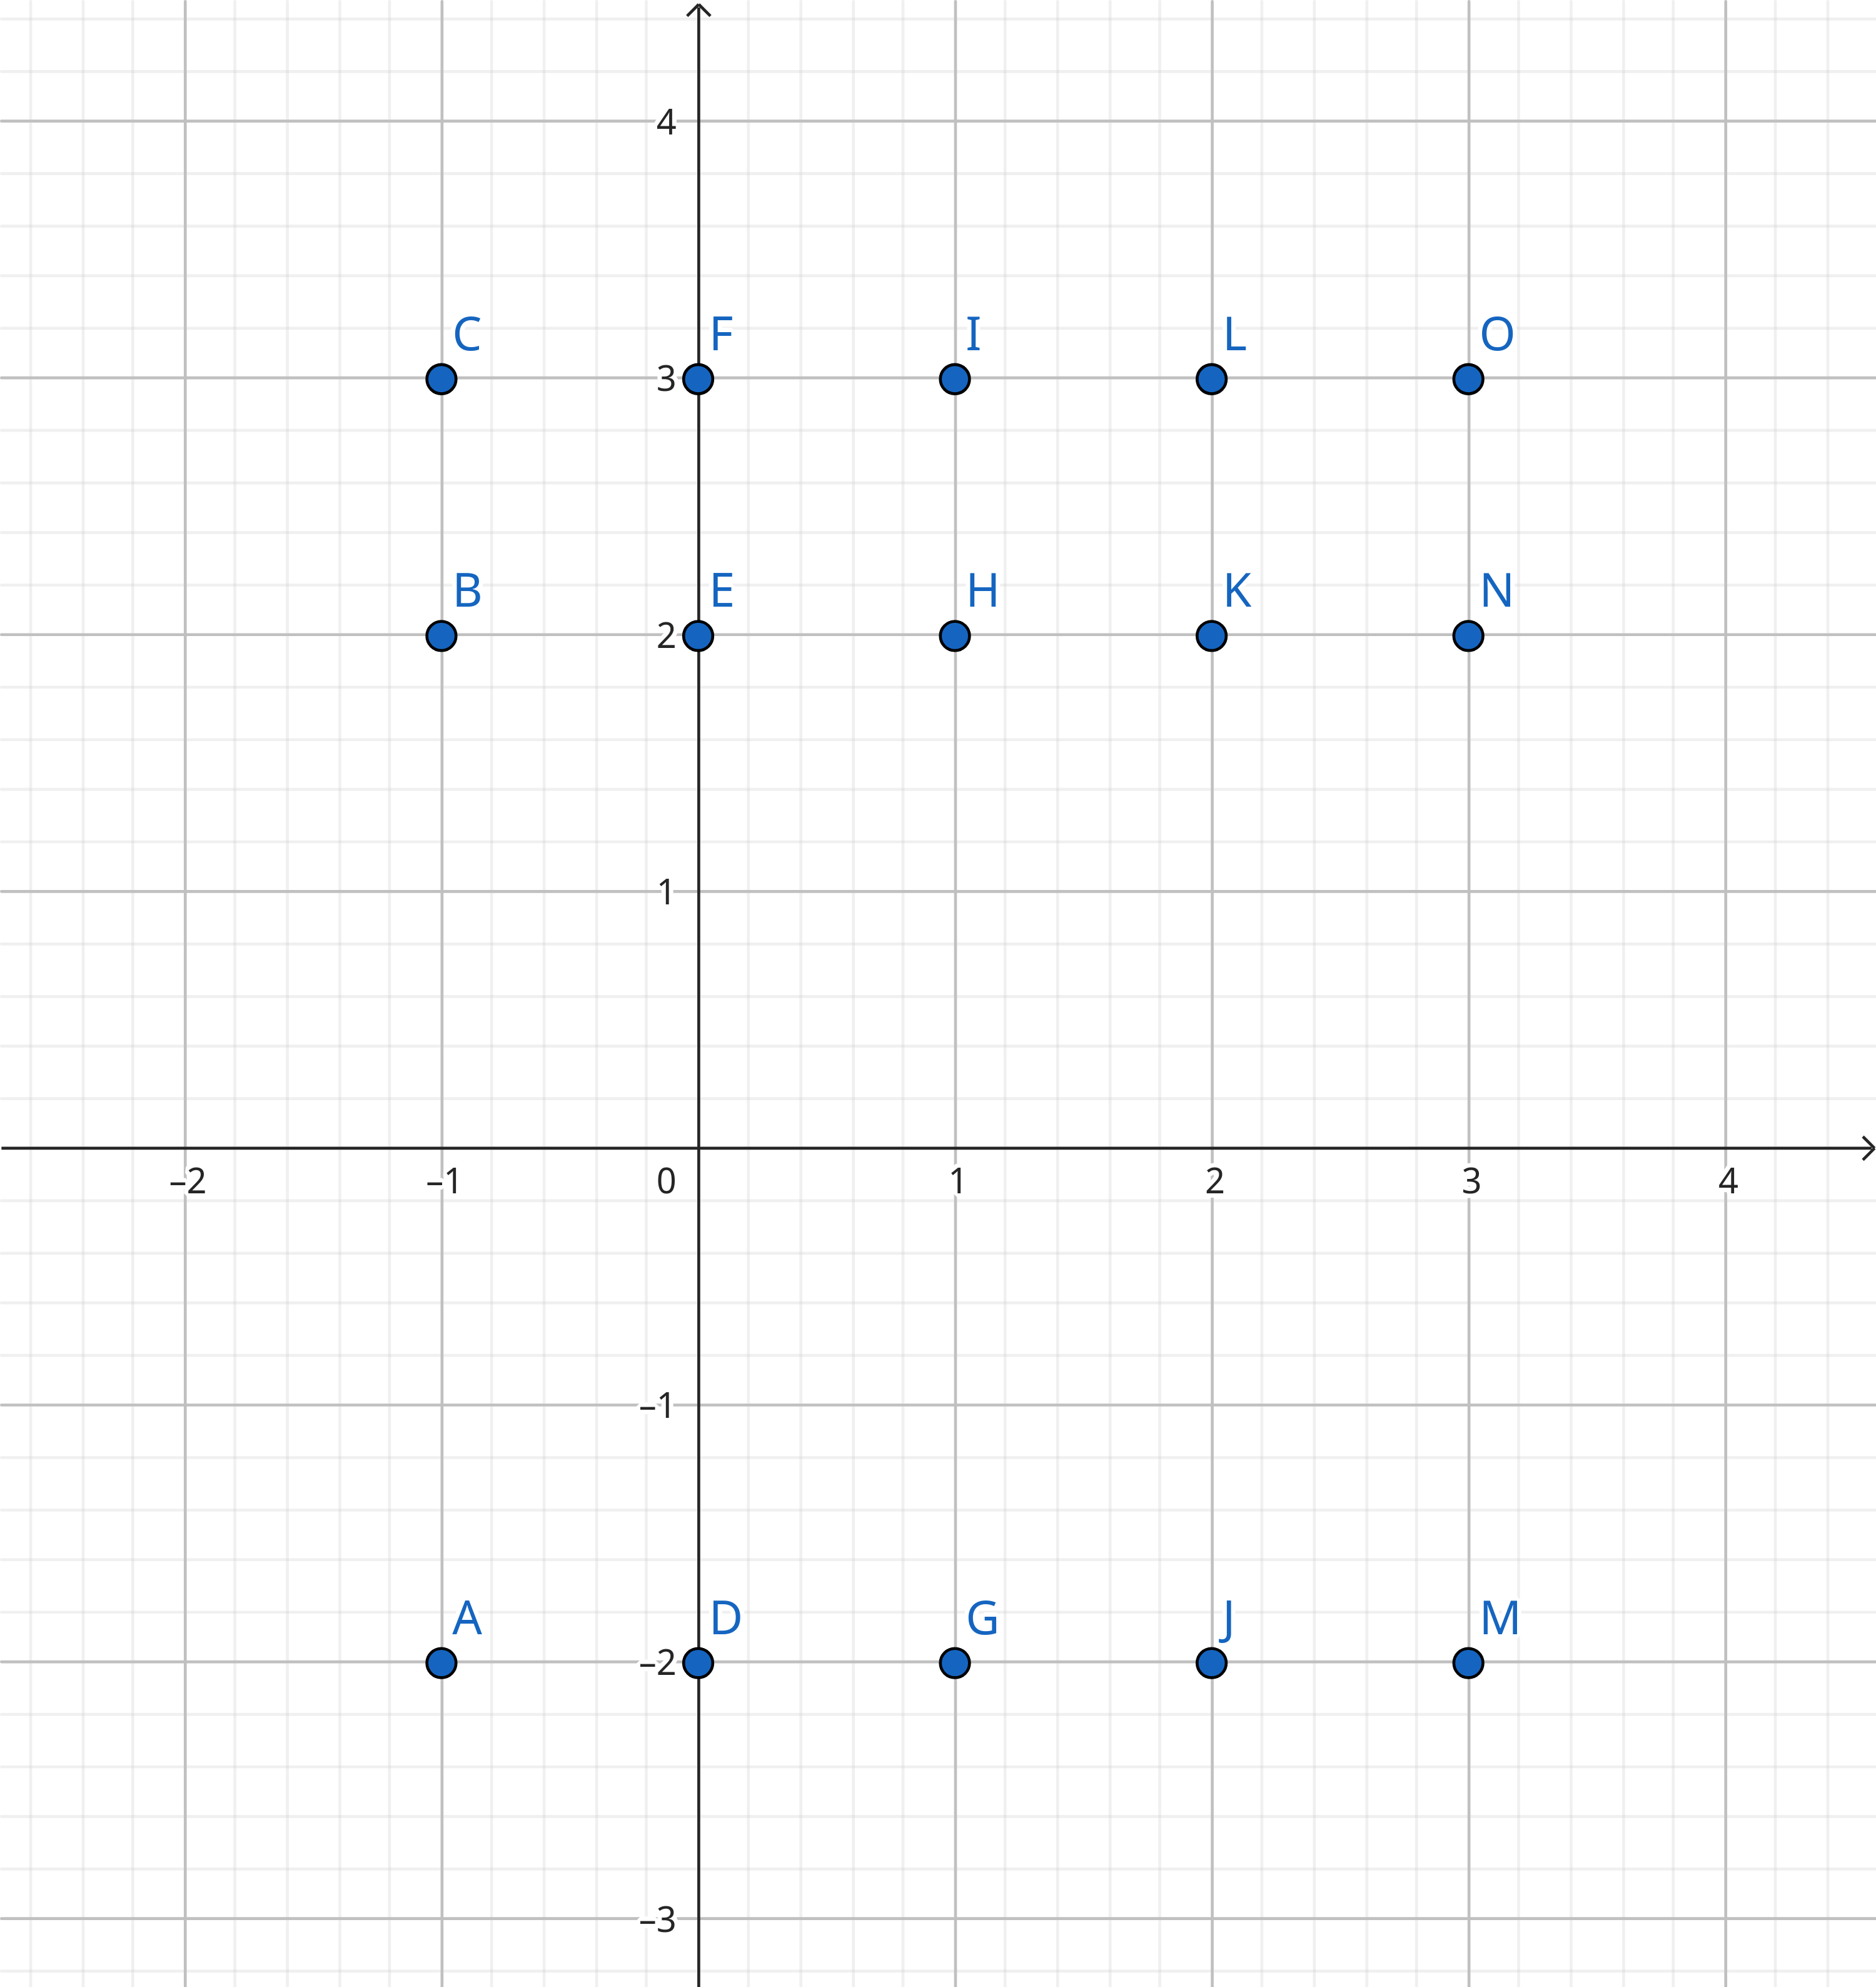
\includegraphics[width=0.55\textwidth]{./assets/abbildung-06-01.png}
            \caption{$[-1,3] \times {-2,2,3}$}
        \end{figure}

    \pagebreak

    \item Schreiben Sie folgende Menge durch Aufz"ahlen all ihrer Elemente
        $(\mathbb{Z} \times \{-1, -2\}) \cap (\{3, 4\} \times \mathbb{Z})$.

        \begin{align*}
            M &= (\mathbb{Z} \times \{-1, -2\}) \cap (\{3, 4\} \times \mathbb{Z}) =\\[5pt]
              &=
              \begin{aligned}[t]
                  \{(x_1, x_2) \text{ : }& x_1 \in \mathbb{Z} \text{, } x_2 \in \{-1, -2\} \text{ und}\\
                                         & x_1 \in \{3, 4\} \text{, } x_2 \in \mathbb{Z}\} =
              \end{aligned}\\
              &= \{(x_1, x_2) \text{ : } x_1 \in \{3, 4\} \text{, } x_2 \in \{-1, -2\}\} =\\[5pt]
              &= \{(3, -1), (3, -2), (4, -1), (4, -2)\}
        \end{align*}
\end{enumerate}


\section{Aufgabe 11}
\setcounter{section}{11}

Pr"ufen Sie die folgenden Aussagen auf ihre G"ultigkeit, und beweisen Sie diese
bzw. widerlegen Sie diese durch ein Gegenbeispiel.

\begin{enumerate}[(a)]
    \item F"ur zwei Mengen $A,B$ mit $A \cap B = \emptyset$ gilt, es gibt keine
        Menge $C$ mit $C \subset A$ und $C \subset B$.
        \begin{align*}
                     &A \cap B = \emptyset \implies \lnot\exists C : C \subset A, C \subset B \\
            \iff     &\exists C : C \subset A, C \subset B \implies A \cap B \neq \emptyset \\[10pt]
                     &\exists C : C \subset A, C \subset B \\
            \iff     &\exists C : \forall x \in C : x \in A, x \in B \\ 
            \implies &\exists a \in A : a \in B \land \exists b \in B : b \in A \implies A \cap B \neq \emptyset \\[10pt]
            \iff     &A \cap B = \emptyset \implies \lnot\exists C : C \subset A, C \subset B
        \end{align*}

    \item F"ur Mengen $M_1, M_2, M_3, C$ gilt $C \subset (M_1 \cup M_2 \cup
        M_3)^c$ genau dann, wenn f"ur alle $j = 1, 2, 3$ $C \cap M_j = \emptyset$
        gilt.
        \begin{align*}
                 &C \subset M^{c(C)} \\
            \iff &C \subset C \setminus M \\
            \implies &\forall_{x \in C} : x \in (C \setminus M) \\
            \iff &\forall_{x \in C} : x \in \{y : y \in C, y \notin M \} \\
            \implies &\forall_{x \in C} : x \notin M \\
            \implies &C \cap M = \emptyset \\
            \\
                 &x \in (M_1 \cup M_2 \cup M_3)^c \\
            \iff &x \in (M_1^c \cap M_2^c \cap M_3^c) \\
            \iff &(x \in M_1^c) \land (x \in M_2^c) \land (x \in M_3^c) \\
            \\
                     &C \subset (M_1 \cup M_2 \cup M_3)^c \\
            \implies &\forall_{x \in C} : x \in (M_1 \cup M_2 \cup M_3)^c \\
            \implies &\forall_{x \in C} : (x \in M_1^c) \land (x \in M_2^c) \land (x \in M_3^c) \\
            \implies &(C \subset M_1^c) \land (C \subset M_2^c) \land (C \subset M_3^c) \\
            \implies &(C \subset M_1 = \emptyset) \land (C \subset M_2 = \emptyset) \land (C \subset M_3 = \emptyset)
        \end{align*}
\end{enumerate}

\section{Aufgabe 13}
\setcounter{section}{13}

\begin{enumerate}[1.]
    \item Wie viele M"oglichkeiten gibt es, 5 unterscheidbare Stifte auf 3 verschiedene
        Schubladen zu verteilen, wenn jede Schublade mehrere Stifte enthalten kann?
        \begin{equation*}
            |\text{Fa}^n_k(uD, mM)| = |\text{Ur}^n_k(mR, mZ)| = n^k = 3^5 = 243
        \end{equation*}

    \item Wie viele M"oglichkeiten gibt es, 8 identische S"u{\ss}igkeiten auf 5
        verschiedene Teller zu verteilen, wobei ein Teller auch leer bleiben
        kann?
        \begin{equation*}
            \begin{aligned}
                |\text{Fa}^n_k(nuD, mM)| &= |\text{Ur}^n_k(oR, mZ)| = \\[10pt]
                                         &= \binom{n + k - 1}{k} = \binom{12}{8} = \\[5pt]
                                         &= \dfrac{12!}{8!(12 - 8)!} = \dfrac{12 \cdot 11 \cdot 10 \cdot 9}{4 \cdot 3 \cdot 2} = 495
            \end{aligned}
        \end{equation*}
\end{enumerate}

\section{Aufgabe 16}
\setcounter{section}{16}

In einer Lotterie werden 6 nummerierte Kugeln aus 49 Kugeln
ungeordnet gezogen. Wie viele Ziehung gibt es, welche die Zahlen
1, 2, 3 enthalten.

Unter der Annahme, dass die Reihenfolge der Ziehungen unerheblich
ist, lässt sich feststellen, dass sich das Ergebnis, bei dem die
ersten drei gezogenen Kugeln die Zahlen 1, 2 und 3 enthalten,
nicht von dem Ergebnis unterscheidet, bei dem diese Kugeln in
einer anderen Reihenfolge gezogen wurden. Es sollte also gen"ugen,
die Anzahl der Möglichkeiten zu berechnen, drei weitere Kugeln zu
ziehen, wenn man davon ausgeht, dass die drei Zielkugeln bereits
gezogen wurden.

\begin{equation*}
    \begin{aligned}
        |\text{Ur}^n_k(oR, oZ)| &= |\text{Fa}^n_k(nuD, oM)| = \\[5pt]
                                &= \binom{n}{k} = \binom{46}{3} = \\[5pt]
                                &= \dfrac{46!}{3!\cdot43!} = \dfrac{46 \cdot 45 \cdot 44}{3 \cdot 2} = 15180
    \end{aligned}
\end{equation*}

\section{Aufgabe 23}
\setcounter{section}{23}

In einer Urne liegen 90 rote Kugeln und 10 wei{\ss}e Kugeln. In einem
Experiment werde 6 mal eine Kugel mit Zur"ucklegen gezogen.

\begin{enumerate}[(a)]
    \item Definieren Sie einen Wahrscheinlichkeitsraum, der dieses Experiment modelliert.
        \begin{equation*}
            |\Omega| = |\text{Ur}_6^{100}(mR, mZ)| = 100^6 = 10^{12}
        \end{equation*}
    \item Definieren Sie auf ihrem W-Raum aus Teil (a) eine
        Zufallsvariable $X$, die die Anzahl der wei{\ss}en Kugeln in diesem
        Experiment z"ahlt, und berechnen Sie damit $P(X = 2)$, $P(X > 4)$ und
        $P(X \leq 2)$.

        Sei $X$ die Zufallsvariable, die die Anzahl der wei{\ss}en Kugeln z"ahlt. Dann gilt:
        \begin{equation*}
            P(X = k) = \left(\dfrac{1}{10}\right)^k
        \end{equation*}
\end{enumerate}

\section{Aufgabe 24}
\setcounter{section}{24}

Es seien $f : X \rightarrow Y$ eine Abbildung und $A, B \subset Y$. Zeigen Sie,
dass folgendes gilt:
\begin{equation*}
    \begin{gathered}
        f^{-1}(A \cap B) = f^{-1}(A) \cap f^{-1}(B)\text{,}\\
        f^{-1}(A \cup B) = f^{-1}(A) \cup f^{-1}(B)
    \end{gathered}
\end{equation*}

\begin{equation*}
    \begin{aligned}
        f^{-1}(A \cap B) &= \{x \in X : f(x) \in \{A \cap B\}\} = \\
                         &= \{x \in X : f(x) \in A \text{ und } f(x) \in B\} = \\
                         &= \{x \in X : f(x) \in A\} \cap \{x \in X : f(x) \in B\} = \\
                         &= f^{-1}(A) \cap f^{-1}(B) \quad \text{\underline{q.e.d.}}
    \end{aligned}
\end{equation*}

\begin{equation*}
    \begin{aligned}
        f^{-1}(A \cup B) &= \{x \in X : f(x) \in \{A \cup B\}\} = \\
                         &= \{x \in X : f(x) \in A \text{ oder } f(x) \in B\} = \\
                         &= \{x \in X : f(x) \in A\} \cup \{x \in X : f(x) \in B\} = \\
                         &= f^{-1}(A) \cup f^{-1}(B) \quad \text{\underline{q.e.d.}}
    \end{aligned}
\end{equation*}

\section{Aufgabe 26}
\setcounter{section}{26}

Beweisen Sie die Aussage $P(A \cup B) = P(A) + P(B) - P(A \cap B)$.
\begin{equation*}
    \begin{aligned}
        A \cup B &= (A \setminus B) \cup (B \setminus A) \cup (A \cap B) \\[5pt]
        P(A \setminus B) &= P(A) - P(A \cap B) \\[5pt]
        P(B \setminus A) &= P(B) - P(A \cap B) \\[5pt]
        P(A \cup B) &= P(A \setminus B) + P(B \setminus A) + P(A \cap B) = \\[5pt]
                    &= (P(A) - P(A \cap B)) + (P(B) - P(A \cap B)) + P(A \cap B) = \\[5pt]
                    &= P(A) + P(B) + P(A \cap B) - P(A \cap B) - P(A \cap B) = \\[5pt]
                    &= P(A) + P(B) - P(A \cap B) \quad \text{\underline{q.e.d.}}
    \end{aligned}
\end{equation*}

\section{Aufgabe 28}
\setcounter{section}{28}

Bestimmen Sie jeweils die Umkehrfunktion folgender Funktionen:
\begin{enumerate}[(a)]
    \item $f : \mathbb{R} \rightarrow \mathbb{R}$, $f(x) = x + 5$, $f^{-1}(x) = x - 5$, $f^{-1}(x) \circ f(x) = x$
    \item $f : (0, \infty) \rightarrow (0, \infty)$, $f(x) = \dfrac{2}{x}$, $f^{-1}(x) = \dfrac{2}{x}$, $f^{-1}(x) \circ f(x) = x$
    \item $f : [0, \infty) \rightarrow [0, \infty)$, $f(x) = x^2 + x$, $f^{-1}(x) = -\dfrac{1}{2} + \sqrt{\dfrac{1}{4} + x}$, $f^{-1}(x) \circ f(x) = x$
\end{enumerate}

\section{Aufgabe 29}
\setcounter{section}{29}

Es seien $M := \{1, 3, 20\}$, $N := \{-1, 4, 0\}$. Bestimmen Sie
$\mathcal{P}(M)$, $\mathcal{P}(N)$, $\mathcal{P}((M \setminus \{3\}) \times (N
\setminus \{-1\}))$.

\begin{enumerate}[(a)]
    \item $\mathcal{P}(M) = \{\emptyset, \{1\}, \{3\}, \{20\}, \{1, 3\},
        \{1, 20\}, \{3, 20\}, \{1, 3, 20\}\}$
    \item $\mathcal{P}(N) = \{\emptyset, \{-1\}, \{4\}, \{0\}, \{-1, 4\},
        \{-1, 0\}, \{4, 0\}, \{-1, 4, 0\}\}$
    \item $\mathcal{P}((M \backslash\{3\}) \times(N \backslash\{-1\})) =
        \begin{aligned}[t]
            \{&\emptyset,\{(1,4)\},\{(1,0)\},\{(20,4)\},\{(20,0)\},\\
              &\{(1,4),(1,0)\},\{(1,4),(20,4)\}, \{(1,4),(20,0)\}, \\
              &\{(1,0),(20,4)\},\{(1,0),(20,0)\},\{(20,4),(20,0)\}, \\
              &\{(1,4),(1,0),(20,4)\},\{(1,4),(1,0),(20,0)\}, \\
              &\{(1,4),(20,4),(20,0)\},\{(1,0),(20,4),(20,0)\}, \\
              &\{(1,4),(1,0),(20,4),(20,0)\}\}
            \end{aligned}$
\end{enumerate}

\section{Aufgabe 31}
\setcounter{section}{31}

Es sei $n \in \mathbb{N}$, bestimmen Sie Formeln zur Berechnung von $|\mathcal{P}(\{\omega, f\})^n|$ und $|\mathcal{P}(\{\omega, f\}^n)|$
\begin{equation*}
    \begin{array}{rcl}
        |\mathcal{P}(\{\omega, f\})^n| &=& |\mathcal{P}(\{\omega, f\})|^n = \\[5pt]
                                       &=& (2^{|\{\omega, f\}|})^n = \\[5pt]
                                       &=& (2^2)^n = \\[5pt]
                                       &=& 4^n \\[10pt]
        |\mathcal{P}(\{\omega, f\}^n)| &=& 2^{|\{\omega, f\}^n|} \\[5pt]
                                       &=& 2^{|\{\omega, f\}|^n} \\[5pt]
                                       &=& 2^{(2^n)}
    \end{array}
\end{equation*}

\pagebreak
\section{Aufgabe 33}
\setcounter{section}{33}

Zeigen Sie mittels Wahrheitstabelle das Folgende:
\begin{enumerate}[a)]
    \item $F_1(A, B) := B \Rightarrow A$ und $F_2(A, B) := \lnot A \Rightarrow
        \lnot B$ sind gleichwertig ($F_1 \Leftrightarrow F_2$)
    \begin{table*}[h]
        \centering
        \begin{minipage}{.29\linewidth}
            \centering
            \begin{tabular}{|c|c|c|}
                \hline
                $A$ & $B$ & $F_1(A, B)$ \\
                \hline
                $w$ & $w$ & $w$ \\
                \hline
                $w$ & $f$ & $w$ \\
                \hline
                $f$ & $w$ & $f$ \\
                \hline
                $f$ & $f$ & $w$ \\
                \hline
            \end{tabular}
        \end{minipage}%
        \begin{minipage}{.29\linewidth}
            \centering
            \begin{tabular}{|c|c|c|}
                \hline
                $A$ & $B$ & $F_2(A, B)$ \\
                \hline
                $w$ & $w$ & $w$ \\
                \hline
                $w$ & $f$ & $w$ \\
                \hline
                $f$ & $w$ & $f$ \\
                \hline
                $f$ & $f$ & $w$ \\
                \hline
            \end{tabular}
        \end{minipage}  \\[15pt]
        \begin{minipage}{1\linewidth}
            \centering
            \begin{tabular}{|c|c|c|}
                \hline
                $F_1(A, B)$ & $F_2(A, B)$ & $F_1(A, B) \Leftrightarrow F_2(A, B)$ \\
                \hline
                $w$ & $w$ & $w$ \\
                \hline
                $w$ & $w$ & $w$ \\
                \hline
                $f$ & $f$ & $w$ \\
                \hline
                $w$ & $w$ & $w$ \\
                \hline
            \end{tabular}
        \end{minipage}
    \end{table*}
    \item $F_3(A, B) := \lnot (A \land B)$ und $F_4(A, B) := \lnot A \lor \lnot
        B$ sind gleichwertig ($F_3 \Leftrightarrow F_4$)
    \begin{table*}[h]
        \centering
        \begin{minipage}{.29\linewidth}
            \centering
            \begin{tabular}{|c|c|c|}
                \hline
                $A$ & $B$ & $F_3(A, B)$ \\
                \hline
                $w$ & $w$ & $f$ \\
                \hline
                $w$ & $f$ & $w$ \\
                \hline
                $f$ & $w$ & $w$ \\
                \hline
                $f$ & $f$ & $w$ \\
                \hline
            \end{tabular}
        \end{minipage}%
        \begin{minipage}{.29\linewidth}
            \centering
            \begin{tabular}{|c|c|c|}
                \hline
                $A$ & $B$ & $F_4(A, B)$ \\
                \hline
                $w$ & $w$ & $f$ \\
                \hline
                $w$ & $f$ & $w$ \\
                \hline
                $f$ & $w$ & $w$ \\
                \hline
                $f$ & $f$ & $w$ \\
                \hline
            \end{tabular}
        \end{minipage}  \\[15pt]
        \begin{minipage}{1\linewidth}
            \centering
            \begin{tabular}{|c|c|c|}
                \hline
                $F_3(A, B)$ & $F_4(A, B)$ & $F_3(A, B) \Leftrightarrow F_4(A, B)$ \\
                \hline
                $f$ & $f$ & $w$ \\
                \hline
                $w$ & $w$ & $w$ \\
                \hline
                $w$ & $w$ & $w$ \\
                \hline
                $w$ & $w$ & $w$ \\
                \hline
            \end{tabular}
        \end{minipage}
    \end{table*}
\end{enumerate}
Somit ist die Gleichwertigkeit der Aussagen bewiesen.

\pagebreak
\section{Aufgabe 35}
\setcounter{section}{35}

Ein neues Online-Lernprogramm soll getestet werden, der laut Anbieter dazu
f"uhren, dass 70\% der Sch"uler eine Verbesserung in ihren Testergebnissen
erzielen. Eine Stichprobe von $n = 40$ Sch"ulern wird zuf"allig ausgew"ahlt und
mit dem Programm geschult. Gegeben sei, dass in der Stichprobe 32 von 40
Sch"ulern eine Verbesserung ihrer Testergebnisse erzielen.

Bestimmen Sie bei einem Signifikanzniveau von $\alpha = 0.05$ f"ur jede
Teilfrage, ob die jeweilige Nullhypothese $H_0$ abgelehnt wird.

\begin{enumerate}[(a)]
    \item Wir nehmen an, dass das Programm tats"achlich eine Erfolgsquote von
        70\% besitzt.
        \begin{enumerate}[i)]
            \item Nullhypothese $H_0$ : $p = 0.7$
            \item Alternativhypothese $H_1$ : $p \neq 0.7$
        \end{enumerate}
        Wir w"ahlen dann das gr"o{\ss}tm"ogliche $k_0, k_1 \in \{0,...,40\}$,
        sodass
        \begin{equation*}
            P(X \leq k_0) + P(X \geq n - k_1) \leq \alpha
        \end{equation*}
        Es ergibt sich damit
        \begin{equation*}
            A := \{0,...,21\} \cup \{34,...,40\} \quad \text{Ablehnungsbereich}
        \end{equation*}
        Daraus folgt mit $T(X) = 32$
        \begin{equation*}
            T(X) \notin A \implies H_0 \text{ wird nicht abgelehnt.}
        \end{equation*}
    \item Das Ziel ist auszuschlie{\ss}en, dass die Erfolgsquote unter 60\% liegt.
        \begin{enumerate}[i)]
            \item Nullhypothese $H_0$ : $p \leq 0.6$
            \item Alternativhypothese $H_1$ : $p > 0.6$
        \end{enumerate}
        Wir w"ahlen dann das gr"o{\ss}tm"ogliche $k_0 \in \{0,...,40\}$,
        sodass
        \begin{equation*}
            P(X \geq n - k_0) \leq \alpha
        \end{equation*}
        Es ergibt sich damit
        \begin{equation*}
            A := \{30,...,40\} \quad \text{Ablehnungsbereich}
        \end{equation*}
        Daraus folgt mit $T(X) = 32$
        \begin{equation*}
            T(X) \in A \implies H_0 \text{ wird abgelehnt.}
        \end{equation*}
    \item Das Ziel ist zu testen, ob die Erfolgsquote m"oglicherweise unter 90\%
        liegt.
        \begin{enumerate}[i)]
            \item Nullhypothese $H_0$ : $p \geq 0.9$
            \item Alternativhypothese $H_1$ : $p < 0.9$
        \end{enumerate}
        Wir w"ahlen dann das gr"o{\ss}tm"ogliche $k_0 \in \{0,...,40\}$,
        sodass
        \begin{equation*}
            P(X \leq k_0) \leq \alpha
        \end{equation*}
        Es ergibt sich damit
        \begin{equation*}
            A := \{0,...,32\} \quad \text{Ablehnungsbereich}
        \end{equation*}
        Daraus folgt mit $T(X) = 32$
        \begin{equation*}
            T(X) \in A \implies H_0 \text{ wird abgelehnt.}
        \end{equation*}
\end{enumerate}

\section{Aufgabe 36}
\setcounter{section}{36}

Nehmen Sie an, dass Sie folgende Aussagen durch einen Widerspruchsbeweis
belegen m"ochten.
\begin{enumerate}[a)]
    \item \textit{Es gibt keine gr"o{\ss}te Primzahl}.

        Hier ist
        \begin{equation*}
            A = (\text{es gibt keine gr"o{\ss}te Primzahl})
            \quad\text{und}\quad
            \lnot A = (\text{es gibt eine gr"o{\ss}te Primzahl})
        \end{equation*}
        Wir nehmen an, dass $\lnot A = wahr$ gilt. Sei $p$ diese gr"o{\ss}te
        Primzahl und seien $1 < p_1 < p_2 < ... < p_n = p$ alle Primzahlen.
        Dann ist $q = p_1 \cdot p_2 \cdot ... \cdot p_n + 1$ eine Primzahl.
        Wenn also $\lnot A = wahr$ gilt, folgt
        \begin{equation*}
            C = (q \leq p) = wahr.
        \end{equation*}
        Da aber sicher gilt $C = falsch$, haben wir den Widerspruch erzeugt,
        und es muss somit $\lnot A = falsch$ gelten.
    \item \textit{F"ur jedes $a \in [0, \infty)$ gibt es mindestens ein $x_0 \in \mathbb{R}$ sodass $x_0^3 - ax_0 = 0$.}

        Hier ist
        \begin{equation*}
            A = (\forall_{a \in [0, \infty)}, \exists_{x_0 \in \mathbb{R}} : x_0^3 - ax_0 = 0)
            \quad\text{und}\quad
            \lnot A = (\exists_{a_0 \in [0, \infty)}, \forall_{x \in \mathbb{R}} : x^3 - a_0x \neq 0)
        \end{equation*}

        \pagebreak
        Wir nehmen an, dass $\lnot A = wahr$ gilt. Sei $a_0 := 0$ und $x_0 := 1$, dann gilt
        \begin{equation*}
            C = (0^3 - 0 \cdot 0 \neq 0) = wahr
        \end{equation*}
        Da aber sicher gilt $C = falsch$, haben wir den Widerspruch erzeugt,
        und es muss somit $\lnot A = falsch$ gelten.
    \item \textit{F"ur jedes Paar $(x_1, x_2)$, $(y_1, y_2) \in \mathbb{R}^2$ gilt:}
        \begin{equation*}
            \sqrt{(x_1 + y_1)^2 + (x_2 + y_2)^2} \leq \sqrt{x_1^2 + x_2^2} + \sqrt{y_1^2 + y_2^2}
        \end{equation*}
        Hier ist
        \begin{equation*}
            A = \left(\forall_{(x_1, x_2), (y_1, y_2) \in \mathbb{R}^2} : \sqrt{(x_1 + y_1)^2 + (x_2 + y_2)^2} \leq \sqrt{x_1^2 + x_2^2} + \sqrt{y_1^2 + y_2^2}\right)
        \end{equation*}
        und
        \begin{equation*}
            \lnot A = \left(\exists_{(x_1, x_2), (y_1, y_2) \in \mathbb{R}^2} : \sqrt{(x_1 + y_1)^2 + (x_2 + y_2)^2} > \sqrt{x_1^2 + x_2^2} + \sqrt{y_1^2 + y_2^2}\right)
        \end{equation*}
        Wir nehmen an, dass $\lnot A = wahr$ gilt. Dann folgt aus der obigen Aussage:
        \begin{equation*}
            \begin{array}{rcl}
                C &=& (\sqrt{(x_1 + y_1)^2 + (x_2 + y_2)^2} > \sqrt{x_1^2 + x_2^2} + \sqrt{y_1^2 + y_2^2}) = wahr \\
                  &\vdots& \\
                C &=& ((x_1y_2 + x_2y_1)^2 < 0) = wahr
            \end{array}
        \end{equation*}
        Da aber sicher gilt $C = falsch$, haben wir den Widerspruch erzeugt,
        und es muss somit $\lnot A = falsch$ gelten.
\end{enumerate}

\section{Aufgabe 38}

Korrigieren Sie die rechte Seite so, dass eine g"ultige Folgerung entsteht.

\begin{enumerate}[(a)]
    \item Mit $f : X \rightarrow Y$ eine Abbildung:

        \quad $f$ ist surjektiv $\Rightarrow$ f"ur jedes $y \in X$ gibt es genau ein $x \in X$ mit $f(x) = y$

        \quad $f$ ist surjektiv $\Rightarrow$ f"ur jedes $y \in Y$ gibt es genau ein $x \in X$ mit $f(x) = y$
    \item Mit $f : X \rightarrow Y$ und $g: Y \rightarrow Z$ zwei Abbildungen:

        \quad $f$ und $g$ sind injektiv $\Rightarrow$ $g \circ f$ ist bijektiv.

        \quad $f$ und $g$ sind injektiv $\Rightarrow$ $g \circ f$ ist injektiv.
    \item Mit $A, B$ zwei Aussagenvariablen:

        \quad $(A \Leftrightarrow B) \Rightarrow (A \Rightarrow \lnot B) \land (B \Rightarrow \lnot A)$

        \quad $(A \Leftrightarrow B) \Rightarrow (A \Rightarrow B) \land (B \Rightarrow A)$
    \item Mit $M$ eine Menge:

        \quad $N \subset M \Rightarrow N \subset \mathcal{P}(M)$

        \quad $N \subset M \Rightarrow N \in \mathcal{P}(M)$
\end{enumerate}


\section{Aufgabe 39}

Der Graph einer Abbildung $f: X \rightarrow Y$ ist laut Definition eine
Teilmenge von $X \times Y$ und damit eine Relation. Pr"ufen Sie welche
Eigenschaften aus Definition 3.3 (im Skript) auf
\begin{itemize}
    \item den Graph einer beliebigen Abbildung,
    \item den Graph einer injektiven Abbildung,
    \item den Graph einer surjektiven Abbildung
\end{itemize}
zutreffen.
\begin{enumerate}
    \item Sei $f: X \rightarrow Y$ eine Abbildung definiert durch $f(X) :=
        \{x^2 : x \in X\} (\subset Y)$ und $G := \{(x, f(x)) : x \in X\}
        (\subset X \times Y)$ der Graph dieser Abbildung. Diese sind durch die
        folgende Tabelle dargestellt:
        \begin{table*}[h]
            \centering
            \begin{tabular}{c|c|c}
                $X$ & $Y$ & $G$ \\
                \hline
                -2 & 4 & (-2, 4) \\
                -1 & 1 & (-1, 1) \\
                0  & 0 & (0,  0) \\
                1  & 1 & (1,  1) \\
                2  & 4 & (2,  4) \\
                   & 5 &
            \end{tabular}
        \end{table*}\\
        Der Graph $G$ hei{\ss}t also:
        \begin{itemize}
            \item \textbf{linkstotal}, weil gilt: $\forall x \in X, \exists y \in Y : (x, y) \in G$
            \item \textbf{rechtseindeutig}, weil gilt: $\forall x \in X$ und $\forall y,z \in Y : (x, y) \in G \land (x, z) \in G \Rightarrow y = z$
        \end{itemize}
    \item Sei $f: X \rightarrow Y$ eine Abbildung definiert durch $f(X) :=
        \{x + 1 : x \in X\} (\subset Y)$ und $G := \{(x, f(x)) : x \in X\}
        (\subset X \times Y)$ der Graph dieser Abbildung. Diese sind durch die
        folgende Tabelle dargestellt:
        \begin{table*}[h]
            \centering
            \begin{tabular}{c|c|c}
                $X$ & $Y$ & $G$ \\
                \hline
                0  & 1 & (0,  1) \\
                1  & 2 & (1,  2) \\
                2  & 3 & (2,  3) \\
                   & 4 &
            \end{tabular}
        \end{table*}

        Der Graph $G$ hei{\ss}t also:
        \begin{itemize}
            \item \textbf{linkstotal}, weil gilt: $\forall x \in X, \exists y \in Y : (x, y) \in G$
            \item \textbf{rechtseindeutig}, weil gilt: $\forall x \in X$ und $\forall y,z \in Y : (x, y) \in G \land (x, z) \in G \Rightarrow y = z$
            \item \textbf{linkseindeutig}, weil gilt: $\forall y \in Y$ und $\forall x,z \in X : (x, y) \in G \land (z, y) \in G \Rightarrow x = z$
        \end{itemize}
    \item Sei $f: X \rightarrow Y$ eine Abbildung definiert durch $f(X) :=
        \{x + 1 : x \in X\} (\subset Y)$ und $G := \{(x, f(x)) : x \in X\}
        (\subset X \times Y)$ der Graph dieser Abbildung. Diese sind durch die
        folgende Tabelle dargestellt:
        \begin{table*}[h]
            \centering
            \begin{tabular}{c|c|c}
                $X$ & $Y$ & $G$ \\
                \hline
                0  & 1 & (0,  1) \\
                1  & 2 & (1,  2) \\
                2  & 3 & (2,  3) \\
            \end{tabular}
        \end{table*} \\
        Der Graph $G$ hei{\ss}t also:
        \begin{itemize}
            \item \textbf{linkstotal}, weil gilt: $\forall x \in X, \exists y \in Y : (x, y) \in G$
            \item \textbf{rechtstotal}, weil gilt: $\forall y \in Y, \exists x \in X: (x, y) \in G$
            \item \textbf{rechtseindeutig}, weil gilt: $\forall x \in X$ und $\forall y,z \in Y : (x, y) \in G \land (x, z) \in G \Rightarrow y = z$
            \item \textbf{linkseindeutig}, weil gilt: $\forall y \in Y$ und $\forall x,z \in X : (x, y) \in G \land (z, y) \in G \Rightarrow x = z$
        \end{itemize}
\end{enumerate}

\section{Aufgabe 42}

Es sei $M := \{(x_1, x_2) \in \mathbb{R}^2 : x_1 \neq 0\}$, und $R \subset M
\times M$ eine Relation definiert durch $R := \{((x_1, x_2), (y_1, y_2)) \in M
\times M : x_2/x_1 = y_2/y_1\}$. Zeigen Sie, dass die Relation $R$ transitiv
ist.

Eine Relation $R$ hei{\ss}t transitiv, wenn
\begin{equation*}
    \forall x,y,z \in M \text{ gilt} : (x, y) \in R \land (y, z) \in R \implies (x, z) \in R
\end{equation*}
Seien $((x_1, x_2), (y_1, y_2)) \in R$ und $((y_1, y_2), (z_1, z_2)) \in R$.
Dann gilt:
\begin{align*}
    &\left(((x_1, x_2), (y_1, y_2)) \in R \Leftrightarrow \dfrac{x_2}{x_1} = \dfrac{y_2}{y_1}\right)
    \land
    \left(((y_1, y_2), (z_1, z_2)) \in R \Leftrightarrow \dfrac{y_2}{y_1} = \dfrac{z_2}{z_1}\right) \\[5pt]
    \iff&
    ((x_1, x_2), (y_1, y_2)) \in R \land ((y_1, y_2), (z_1, z_2)) \in R
    \Leftrightarrow
    \dfrac{x_2}{x_1} = \dfrac{y_2}{y_1} \land \dfrac{y_2}{y_1} = \dfrac{z_2}{z_1}
\end{align*}
Und wenn $\dfrac{x_2}{x_1} = \dfrac{y_2}{y_1} \land \dfrac{y_2}{y_1} =
\dfrac{z_2}{z_1} \Rightarrow \dfrac{x_2}{x_1} = \dfrac{z_2}{z_1}$ gilt, gilt auch
\begin{align*}
    &((x_1, x_2), (y_1, y_2)) \in R \land ((y_1, y_2), (z_1, z_2)) \in R
    \Rightarrow
    \dfrac{x_2}{x_1} = \dfrac{z_2}{z_1} \\[5pt]
    \iff&
    ((x_1, x_2), (y_1, y_2)) \in R \land ((y_1, y_2), (z_1, z_2)) \in R
    \Rightarrow
    ((x_1, x_2), (z_1, z_2)) \in R
\end{align*}
Daher ist die Relation $R$ transitiv, was zu beweisen war.

\section{Aufgabe 44}

Es sei $M$ eine Menge, $R \subset M \times M$ eine "Aquivalenzrelation und $x,
y \in M$. Zeigen Sie, dass dann entweder $[x]_R = [y]_R$ oder $[x]_R \cap [y]_R
= \emptyset$ gilt.

Zu zeigen ist, dass die Aussage
\begin{align*}
    (R \subset M \times M) \land (x, y \in M) \Rightarrow ([x]_R = [y]_R) \xor ([x]_R \cap [y]_R = \emptyset)
\end{align*}
gilt.

Die Aussage $(R \subset M \times M) \land (x, y \in M)$ ist immer wahr laut der
Aufgabenstellung. Es bleibt also nur noch zu beweisen, dass der rechte Teil
der Implikation auch gilt.
\begin{equation*}
    \begin{array}{rrcrcl}
                         &([x]_R = [y]_R) &\xor&           ([x]_R \cap [y]_R    = \emptyset) &\overset{!}{=}& w \\[15pt]
        \iff             &([x]_R = [y]_R) &\lor&           ([x]_R \cap [y]_R    = \emptyset) &\land& \\[5pt]
             &\land\ \lnot([x]_R = [y]_R) &\lor&      \lnot([x]_R \cap [y]_R    = \emptyset) &\overset{!}{=}& w \\[5pt]
        \iff &\lnot([x]_R \neq [y]_R)     &\lor&           ([x]_R \cap [y]_R    = \emptyset) &\land& \\[5pt]
             &\land\ \lnot([x]_R = [y]_R) &\lor&           ([x]_R \cap [y]_R \neq \emptyset) &\overset{!}{=}& w \\[5pt]
        \iff             &([x]_R \neq [y]_R) &\Rightarrow& ([x]_R \cap [y]_R    = \emptyset) &\land& \\[5pt]
                  &\land\ ([x]_R = [y]_R)    &\Rightarrow& ([x]_R \cap [y]_R \neq \emptyset) &\overset{!}{=}& w
     \end{array}
\end{equation*}
Dies bringt zwei weitere Implikationen:
\begin{enumerate}[i)]
    \item $[x]_R \neq [y]_R \Rightarrow ([x]_R \cap [y]_R = \emptyset)$ : wenn
        "Aquivalenzklassen $[x]_R$ und $[y]_R$ ungleich sind, dann sind sie
        komplett unterschiedlich.

        Nehmen wir an, dass die Aussage $([x]_R \cap [y]_R = \emptyset)$ nicht wahr ist.
        Dann gilt
        \begin{equation*}
            \begin{array}{rc}
                        &[x]_R \cap [y]_R \neq \emptyset \Leftrightarrow (\exists_{z \in M} : z \in [x]_R \land z \in [y]_R)  \\[5pt]
                \implies& (x, z) \in R \land (y, z) \in R \Rightarrow (x, y) \in R
            \end{array}
        \end{equation*}
        Daraus folgt, dass $x$ und $y$ miteinander verbunden sind und geh"oren
        daher zur gleichen "Aquivalenzklassen. Das hei{\ss}t
        \begin{equation*}
            \begin{array}{rlcl}
                      &\phantom{\lnot}[x]_R \cap [y]_R \neq \emptyset &\implies& \phantom{\lnot}[x]_R = [y]_R \\[5pt]
                \iff  &\lnot[x]_R \cap [y]_R =    \emptyset &\implies& \lnot[x]_R \neq [y]_R \\[5pt]
                \iff  &\phantom{\lnot}[x]_R \neq [y]_R                &\implies& \phantom{\lnot}[x]_R \cap [y]_R =    \emptyset \quad \text{\underline{q.e.d.}}
            \end{array}
        \end{equation*}
    \item $[x]_R = [y]_R \Rightarrow ([x]_R \cap [y]_R \neq \emptyset)$ : wenn
        "Aquivalenzklassen $[x]_R$ und $[y]_R$ gleich sind, dann bilden sie
        eine nicht-leere Schnittmenge.

        Die Aussage ist allgemein f"ur alle Mengen richtig und braucht keinen
        formellen Beweis.
\end{enumerate}

Daraus folgt:
\begin{equation*}
    \begin{array}{rrcrcl}
        \iff             &([x]_R \neq [y]_R) &\Rightarrow& ([x]_R \cap [y]_R    = \emptyset) &\land& \\[5pt]
                  &\land\ ([x]_R = [y]_R)    &\Rightarrow& ([x]_R \cap [y]_R \neq \emptyset) &=& w
     \end{array}
\end{equation*}
was zu beweisen war $\square$

\section{Aufgabe 45}

Es sei $\Omega = \{0, 1\}^3$ mit $P(\{\omega\}) = \dfrac{1}{8}$ $(\omega \in \Omega)$ unser W-Raum. Dann gilt
\begin{equation*}
    \Omega = \{(0, 0, 0), (0, 0, 1), (0, 1, 0), (0, 1, 1), (1, 0, 0), (1, 0, 1), (1, 1, 0), (1, 1, 1)\}
\end{equation*}
Daraus ergibt sich das Folgende:
\begin{enumerate}[i)]
    \item $P(X = 4 | Y = f_1) = \dfrac{6}{8} = \dfrac{3}{4}$
    \item $P(X = 4 | Y = f_2) = \dfrac{2}{8} = \dfrac{1}{4}$
    \item $P(X = 4 | Y = f_3) = \dfrac{3}{8}$
\end{enumerate}
Gem"a{\ss} der Bayes-Formel (6.49 im Skript) gilt
\begin{equation*}
    P(Y = f_l | X = 4) = \dfrac{P(X = 4 | Y = f_l)P(Y = f_l)}{\sum_{j = 1}^nP(X = 4 | Y = f_j)P(Y = f_j)}
\end{equation*}
Daraus folgt
\begin{enumerate}[i)]
    \item $\begin{aligned}[t]
            P(Y = f_1 | X = 4) &= \dfrac{P(X = 4 | Y = f_1)P(Y = f_1)}{\sum_{j = 1}^3P(X = 4 | Y = f_j)P(Y = f_j)}  \\[5pt]
                               &= \dfrac{6/8 \cdot 1/3}{6/8 \cdot 1/3 + 2/8 \cdot 1/3 + 3/8 \cdot 1/3} = \dfrac{6}{11}
        \end{aligned}$ \\[5pt]
    \item $\begin{aligned}[t]
            P(Y = f_2 | X = 4) &= \dfrac{P(X = 4 | Y = f_2)P(Y = f_2)}{\sum_{j = 1}^3P(X = 4 | Y = f_j)P(Y = f_j)}  \\[5pt]
                               &= \dfrac{2/8 \cdot 1/3}{6/8 \cdot 1/3 + 2/8 \cdot 1/3 + 3/8 \cdot 1/3} = \dfrac{2}{11}
        \end{aligned}$ \\[5pt]
    \item $\begin{aligned}[t]
            P(Y = f_3 | X = 4) &= \dfrac{P(X = 4 | Y = f_3)P(Y = f_3)}{\sum_{j = 1}^3P(X = 4 | Y = f_j)P(Y = f_j)}  \\[5pt]
                               &= \dfrac{3/8 \cdot 1/3}{6/8 \cdot 1/3 + 2/8 \cdot 1/3 + 3/8 \cdot 1/3} = \dfrac{3}{11}
        \end{aligned}$
\end{enumerate}

\section{Aufgabe 47}
\begin{enumerate}
    \item $[3]_8 + [9]_8 + [-1]_8 = [3]_8 + [1]_8 + [7]_8 = [11]_8 = [3]_8$
    \item $[3]_5 + [1]_5 + [10]_5 = [3]_5 + [1]_5 + [0]_5 = [4]_5$
    \item $[7]_7 \cdot [6]_7 \cdot [-1]_7 = [0]_7 \cdot [6]_7 \cdot [6]_7 = [0]_7$
    \item $([6]_{13} \cdot [-5]_{13}) + [-3]_{13} = ([6]_{13} \cdot [8]_{13}) + [10]_{13} = [58]_{13} = [6]_{13}$
    \item $([8]_{-2} \cdot [6]_{-2}) + [-1]_{-2} = ([0]_{-2} \cdot [0]_{-2}) + [-1]_{-2} = [1]_{-2}$
\end{enumerate}

\section{Aufgabe 51}
\setcounter{section}{51}

\begin{enumerate}[(a)]
    \item $P(X \leq k) = \sum_{i = 0}^kp(1 - p)^i = p\sum_{i = 0}^k(1 - p)^i = p \cdot \dfrac{1 - (1 - p)^{k + 1}}{1 - (1 - p)} = 1 - (1 - p)^{k + 1}$
    \item $f(p) = p(1 - p)^2 = p^3 - 2p^2 + p\text{;  } f'(p) = 3p^2 - 4p + 1\text{;  } f''(p) = 6p - 4 \\[5pt]
            f'(p) = 0 \iff p = 1 \lor p = 1/3a \\[5pt]
            f''(1/3) < 0 \iff p = 1/3$
\end{enumerate}

\section{Aufgabe 52}
\setcounter{section}{52}

\begin{enumerate}[(a)]
    \item $P(1 \leq X \leq 5) = \sum_{k = 1}^5P(X = k)$
    \item $P(X + Y \leq 3) = P(X = 0 \land Y \leq 3) + P(X = 1 \land Y \leq 2) + P(X = 2 \land Y \leq 1)$
    \item $P(X > 4 \land Y < 2) = P(X > 4) \cdot P(Y < 2) = (1 - P(X \leq 4)) \cdot P(Y < 2)$
\end{enumerate}

\section{Aufgabe 53}
\setcounter{section}{53}

Gegeben ist eine Urne, die vier Kugeln enth"alt. Die Kugeln sind mit den Zahlen
1, 2, 3, 4 nummeriert. Es werden zwei Kugeln gleichzeitig und zuf"allig aus der
Urne gezogen, und anschlie{\ss}end werden die Nummern der beiden gezogenen
Kugeln addiert.
\begin{enumerate}
    \item Bestimmen Sie die m"oglichen Werte, die die Summe der gezogenen
        Kugelnummern annehmen kann, und berechnen Sie die Wahrscheinlichkeit
        f"ur jede dieser Summen.

        Sei $X : \Omega \rightarrow \mathbb{R}$ die Zufallsvariable, die die
        Summe der beiden gezogenen Kugelnummern annehmt, und $(\Omega, P)$ ein
        W-Raum, dann gilt:
        \begin{equation*}
            |\Omega| = \binom{4}{2} = 6 \quad\text{und}\quad P = \dfrac{1}{6}
        \end{equation*}
        \begin{table*}[h]
            \centering
            \begin{tabular}{c|c}
                $x_i$ & $P(X = x_i)$ \\
                \hline
                3 & 0.16 \\
                4 & 0.16 \\
                5 & 0.33 \\
                6 & 0.16 \\
                7 & 0.16 \\
            \end{tabular}
        \end{table*}
    \item Berechnen Sie den Erwartungswert der Summe der gezogenen Kugelnummern.
        \begin{equation*}
            E(X) = \dfrac{1}{6} \cdot (3 + 4 + 6 + 7) + \dfrac{1}{3} \cdot 5 = 5
        \end{equation*}
\end{enumerate}

\section{Aufgabe 54}

Es sei $(G, *)$ eine Gruppe. Zeigen Sie das Folgende:
\begin{enumerate}[(a)]
    \item F"ur alle $x, y \in G$ gilt $(x * y)^{-1} = y^{-1} * x^{-1}$ \\[5pt]
        Sei $A = ((x * y)^{-1} = y^{-1} * x^{-1})$. Dann gilt $\lnot A = ((x * y)^{-1} \neq y^{-1} * x^{-1})$.

        \textbf{Beweis.} Wir nehmen an, dass die Aussage $\lnot A = wahr$ gilt.
        Daraus folgt:
        \begin{equation*}
            \begin{array}{rrcll}
                        &(x * y)^{-1} &\neq& y^{-1} * x^{-1} &| * x * y \\[5pt]
                \implies&(x * y)^{-1} * (x * y) &\neq& y^{-1} * x^{-1} * x * y \\[5pt]
                \implies&e &\neq& y^{-1} * e * y \\[5pt]
                \implies&e &\neq& y^{-1} * y \\[5pt]
                \implies&e &\neq& e
            \end{array}
        \end{equation*}
        Da aber sicher gilt $(e \neq e) = falsch$, haben wir unser Widerspruch
        erzeugt, und es muss somit $\lnot A = falsch$ gelten.
    \item Die Gruppe ist genau dann kommutativ, wenn f"ur alle $x, y \in G$
        gilt $x * y * x^{-1} * y^{-1} = e$ \\[5pt]
        \textbf{Beweis.}
        Eine Gruppe $G$ hei{\ss}t kommutativ, wenn $\forall x, y \in G$ gilt:
            \begin{equation*}
                x * y = y * x
            \end{equation*}
        \begin{enumerate}[i)]
            \item Wenn $(x * y) = (y * x)$ gilt, folgt
                \begin{equation*}
                    \begin{array}{rrcll}
                                 &e &=& e &| * x * x^{-1} * y * y^{-1}\\[5pt]
                        \implies &e * x * x^{-1} * y * y^{-1} &=& e * x * x^{-1} * y * y^{-1} & \\[5pt]
                        \implies &x * x^{-1} * y * y^{-1} &=& e \\[5pt]
                        \implies &x * y * x^{-1} * y^{-1} &=& e
                    \end{array}
                \end{equation*}
                Somit gilt f"ur alle $x, y \in G$
                $$(x * y) = (y * x) \Rightarrow x * y * x^{-1} * y^{-1} = e$$

            \item Wenn $x * y * x^{-1} * y^{-1} = e$ gilt, folgt
                \begin{equation*}
                    \begin{array}{rrcll}
                                 &x * y * x^{-1} * y^{-1} &=& e &| * y \\[5pt]
                        \implies &x * y * x^{-1} * y^{-1} * y &=& e * y \\[5pt]
                        \implies &x * y * x^{-1} &=& y &| * x \\[5pt]
                        \implies &x * y * x^{-1} * x &=& y * x \\[5pt]
                        \implies &x * y &=& y * x
                    \end{array}
                \end{equation*}
                Somit gilt f"ur alle $x, y \in G$
                $$x * y * x^{-1} * y^{-1} = e \Rightarrow (x * y) = (y * x)$$
        \end{enumerate}
        Aus i) und ii) entsteht die folgende Aussageformel:
        \begin{gather*}
            ((x * y) = (y * x) \Rightarrow (x * y * x^{-1} * y^{-1} = e))\ \land \\
            \land\ ((x * y * x^{-1} * y^{-1} = e) \Rightarrow (x * y) = (y * x))
        \end{gather*}
        oder
        \begin{equation*}
            (x * y) = (y * x) \Leftrightarrow (x * y * x^{-1} * y^{-1} = e) \quad \text{\underline{q.e.d.}}
        \end{equation*}
\end{enumerate}

\section{Aufgabe 60}
\begin{enumerate}[(a)]
    \item $\begin{aligned}[t]
            \prod_{i = 1}^{n} (a_i \cdot b_{n - i + 1}) &= a_1 \cdot b_{n} \cdot a_2 \cdot b_{n - 1} \cdot ... \cdot a_{n} \cdot b_{1} = (a_1 \cdot a_2 \cdot ... \cdot a_n) \cdot (b_1 \cdot b_2 \cdot ... \cdot b_n) = \\
                                                        &= \prod_{i = 1}^n(a_i) \cdot \prod_{i = 1}^2(b_i) \quad \text{\underline{q.e.d.}}
        \end{aligned}$
    \item $\begin{aligned}[t]
            \sum_{i = 0}^n((a_i + b_i)^2) &= (a_1 + b_1)^2 + (a_2 + b_2)^2 + ... + (a_n + b_n)^2 = \\
                                          &= (a_1^2 + 2a_1b_1 + b_1^2) + (a_2^2 + 2a_2b_2 + b_2^2) + ... + (a_n^2 + 2a_nb_n + b_n^2) = \\[5pt]
                                          &= (a_1^2 + a_2^2 + ... + a_n^2) + 2(a_1b_1 + a_2b_2 + ... + a_nb_n) + (b_1^2 + b_2^2 + ... + b_n^2) = \\[5pt]
                                          &= \sum_{i = 1}^n(a_i^2) + 2\sum_{i = 1}^n(a_ib_i) + \sum_{i = 1}^n(b_i^2) = \\[5pt]
                                          &= \sum_{i = 1}^n(a_i^2 + 2a_ib_i + b_i^2) \neq (\sum_{i = 1}^n(a_i) + \sum_{i = 1}^n(b_i))^2
        \end{aligned}$
\end{enumerate}

\pagebreak
\section{Aufgabe 62}

Zeigen Sie durch vollst"andige Induktion, dass f"ur $n \in \mathbb{N}$ folgendes gilt:
\begin{equation*}
    \sum_{\nu = 1}^n\nu^3 = \dfrac{1}{4}n^2(n + 1)^2
\end{equation*}
\begin{enumerate}[i)]
    \item \textbf{Induktionsanfang:} Zeigen wir, dass die Aussage f"ur $n = 1$ gilt
        \begin{align*}
            1^3 &= \dfrac{1}{4} \cdot 1^2(1 + 1)^2 \\[5pt]
            1 &= \dfrac{1}{4} \cdot 4 \\[5pt]
            1 &= 1
        \end{align*}
    \item \textbf{Induktionsannahme:} Wir nehmen an, dass die Aussage f"ur ein allgemeines $n_k$
        \begin{align*}
            1^3 + 2^3 + ... + k^3 = \dfrac{1}{4} \cdot k^2(k + 1)^2
        \end{align*}
    \item \textbf{Induktionsschritt:} Zeigen wir, dass unter der
        Induktionsannahme f"ur $n_k$, folgt, dass diese Aussage auch f"ur $n_{k
        + 1}$ gilt
        \begin{align*}
            1^3 + 2^3 + ... + k^3 + (k + 1)^3 &= \dfrac{1}{4} \cdot (k + 1)^2(k + 2)^2 \\[5pt]
            \dfrac{1}{4} \cdot k^2(k + 1)^2 + (k + 1)^3 &= \dfrac{1}{4} \cdot (k + 1)^2(k + 2)^2 \\[5pt]
            (k + 1)^2 \cdot \left(\dfrac{1}{4} \cdot k^2 + (k + 1)\right) &= \dfrac{1}{4} \cdot (k + 1)^2(k + 2)^2 \\[5pt]
            (k + 1)^2 \cdot \left(\dfrac{1}{4} \cdot k^2 + \dfrac{1}{4} \cdot (4k + 4)\right) &= \dfrac{1}{4} \cdot (k + 1)^2(k + 2)^2 \\[5pt]
            \dfrac{1}{4} \cdot (k + 1)^2 (k^2 + 4k + 4) &= \dfrac{1}{4} \cdot (k + 1)^2(k + 2)^2 \\[5pt]
            \dfrac{1}{4} \cdot (k + 1)^2 (k + 2)^2 &= \dfrac{1}{4} \cdot (k + 1)^2(k + 2)^2 \\[5pt]
        \end{align*}
\end{enumerate}

\section{Aufgabe 72}

\begin{enumerate}[(a)]
    \item In der Mensa stehen 6 Men"us zur Auswahl und Sie gehen mit 6 weiteren
        Kommilitonen zum Essen, von denen jeder genau ein Men"u nimmt. Wie
        viele m"ogliche Men"uauswahlen k"onnen dabei getroffenen werden? Es
        soll dabei alleine die Auswahl, und nicht die Zuordnung zu den
        einzelnen Personen unterschieden werden.
        \begin{align*}
            \text{Ur}_6^6(mZ, oR) &= \binom{6 + 6 - 1}{6} = \binom{11}{6} = \dfrac{11!}{6!\cdot5!} = 462
        \end{align*}
    \item Zeigen Sie, dass f"ur $n, \nu \in \mathbb{N}$, $n \geq \nu$ gilt
        \begin{align*}
            \binom{n + 1}{\nu} &= \binom{n}{\nu - 1} + \binom{n}{\nu} \\[5pt]
                               &= \dfrac{n!}{(\nu - 1)!(n - \nu + 1)!} + \dfrac{n!}{\nu!(n - \nu)!} \\[5pt]
                               &= \dfrac{n!\nu + n!(n - \nu + 1))}{\nu!(n - \nu + 1)!} \\[5pt]
                               &= \dfrac{n!(n + 1)}{\nu!(n - \nu + 1)!} \\[5pt]
                               &= \binom{n + 1}{\nu}
        \end{align*}
\end{enumerate}


\end{document}
